\documentclass[11pt,a4paper]{article}
\usepackage{ctex}  % 支持中文
\usepackage{cite}
\usepackage{amsmath,amssymb,amsfonts}
\usepackage{graphicx}
\usepackage{textcomp}
\usepackage{xcolor}
\usepackage{algorithm}
\usepackage{algorithmic}
\usepackage{geometry}
\usepackage{authblk}

% 设置页面边距
\geometry{
    a4paper,
    top=2.5cm,
    bottom=2.5cm,
    left=2.5cm,
    right=2.5cm
}

% 设置行距
\linespread{1.3}

\begin{document}

\title{\Large 高维稀疏数据的文本分类研究}

\author{xxx}
\affil{上海交通大学\\学号: xxx\\邮箱: xxx}

\date{}  % 如果需要日期,删除这一行

\maketitle

\begin{abstract}
本研究探讨了一个20类文本分类任务,重点处理高维稀疏数据。我们实现并比较了多种机器学习方法,包括逻辑回归(Logistic Regression)、支持向量机(SVM)和MLP。实验表明,适当的特征处理和模型选择对高维稀疏数据的分类性能有显著影响。最佳模型在测试集上取得了令人满意的分类结果。
\end{abstract}

\section{引言}
文本分类是自然语言处理中的基础任务。本项目聚焦于一个匿名的文本分类数据集,包含了11,314个训练样本和7,532个测试样本,每个样本被表示为一个10,000维的特征向量。主要挑战包括:
\begin{itemize}
    \item 高维度(10,000个特征)
    \item 数据稀疏性
    \item 多类分类(20个类别)
\end{itemize}

\section{数据处理技术}
\subsection{数据分析}
对数据集的初步分析显示:
\begin{itemize}
    \item 基本特征:训练集大小:11,314个样本;特征维度:10,000;类别数:20
    \item 数据格式:稀疏矩阵(CSR格式)
    \item 稀疏度:特征矩阵中超过99\%的元素为零
    \item 每个样本的非零特征平均数:约45
\end{itemize}
\subsubsection{类别不平衡分析}
类别分布呈现出一定的偏斜,某些类别的样本数少于其他类别。尽管在大多数情况下,样本数相对均衡,但某些类别(如类别19和类别0)的样本数明显少于其他类别(将近少了一半)。这种不平衡可能会对模型的分类性能产生影响,尤其是当模型倾向于偏向于样本数较多的类别时。

为了更好地理解数据集的类别不平衡情况,我生成了类别分布图,如下所示:

\begin{figure}[htbp]
    \centering
    \includegraphics[width=0.8\textwidth]{../picture/class_distribution.png}
    \caption{训练集类别分布图}
    \label{fig:class_distribution}
\end{figure}

从图中可以看到,类别19的样本数最少,只有377个样本,而类别10则具有最多的样本,达到600个样本。这种类别不平衡可能会导致模型在预测少数类别时出现偏差,因此我们在训练过程中采用了处理不平衡数据的方法,包括通过调整类别权重来平衡每个类别的重要性。


\subsubsection{稀疏度分析}

在本研究中,训练数据集的稀疏度为 0.9915,即99.15\% 的矩阵元素为零。这表明数据集是高度稀疏的,大部分特征在每个样本中都不包含有效信息。以下是对训练sparsity的详细分析和可视化结果:

\begin{itemize}
    \item \textbf{每个样本的非零特征数}:从样本的角度看:平均每个样本有 84.51 个非零特征,最大为 1600(略高于维数的10\%),最小为 6,这表明大部分样本所含有效特征都相对较少。
    \item \textbf{每个特征的非零出现次数}:从特征的角度看:每个特征平均出现 95.61 次,最常出现的特征出现在 5272 个样本中,最不常出现的特征则没有在任何样本中出现。这可能是由于某些特征在所有文档中都不重要(例如停用词)。
\end{itemize}

我们进一步通过python脚本可视化了数据的稀疏度分布:

\begin{enumerate}
    \begin{figure}[htbp]
        \centering
        \begin{minipage}{0.48\textwidth}
            \centering
            \includegraphics[width=\textwidth]{../picture/non-zero_features_per_example.png}
            \caption{每个样本的非零特征数分布}
            \label{fig:non_zero_features_per_sample}
        \end{minipage}
        \hfill
        \begin{minipage}{0.48\textwidth}
            \centering
            \includegraphics[width=\textwidth]{../picture/non-zero_occurrences_per_example.png}
            \caption{每个特征的非零出现次数分布}
            \label{fig:non_zero_occurrences_per_feature}
        \end{minipage}
        
        \vspace{0.5cm}
        
        \begin{minipage}{0.48\textwidth}
            \centering
            \includegraphics[width=\textwidth]{../picture/sparsity_distribution_for_examples.png}
            \caption{每个样本的稀疏度分布}
            \label{fig:sparsity_per_sample}
        \end{minipage}
        \hfill
        \begin{minipage}{0.48\textwidth}
            \centering
            \includegraphics[width=\textwidth]{../picture/sparsity_distribution_for_features.png}
            \caption{每个特征的稀疏度分布}
            \label{fig:sparsity_per_feature}
        \end{minipage}
    \end{figure}

    \item \textbf{每个样本的非零特征数分布}:这张图显示了每个样本中非零特征的数量分布。可以看到绝大多数样本的非零特征数都小于100。
    \item \textbf{每个特征的非零出现次数分布}:这张图展示了每个特征在所有样本中出现的次数分布。将近有80\%的特征非零出现次数小于100。
    \item \textbf{每个样本的稀疏度分布}:稀疏度定义为每个样本的零元素占比,分布情况如图所示。可以看到绝大多数样本的稀疏度都大于98\%。
    \item \textbf{每个特征的稀疏度分布}:这张图显示了特征在所有样本中的稀疏度分布。大多数特征的稀疏度都在95\%以上,即只出现在了5\%左右的样本中。
\end{enumerate}

\textbf{结论}:

\begin{itemize}
    \item \textbf{高稀疏性}:训练集具有极高的稀疏性,大多数样本所含非零特征小于1\%,大多数特征只在5\%左右的样本中出现。这种高稀疏性在文本分类中相对常见。可以通过稀疏矩阵格式有效地存储这些数据,以减少内存开销。同时为了削弱维数灾难,以及增加模型的泛化能力,可以使用PCA,LDA等方法进行数据降维。
    
    \item \textbf{样本差异性}:尽管大多数样本具有相对较少的非零特征(平均 84.51 个非零特征),但一些样本包含了大量的有效特征,最多达到 1600 个非零特征。这表明样本之间在文本长度和信息密度上的差异较大,需要对不同类型的样本采用不同的处理方法。
    
    \item \textbf{特征分布}:某些特征在所有样本中都非常常见(例如最多出现 5272 次),而另一些特征几乎没有出现(最少为 0)。这表明在特征空间中,一些特征在所有样本中都是重要的,而一些特征可能完全没有贡献,需要进行特征选择或去除不相关特征。
    
    \item \textbf{数据优化方向}:
    \begin{itemize}
        \item \textbf{特征选择}:通过去除低频或完全不出现的特征来减少特征空间的维度,优化模型训练。
        \item \textbf{样本平衡}:对稀疏的短文本样本和包含大量信息的长文本样本,可以考虑不同的采样方法或者模型架构来适应不同类型的文本数据。
        \item \textbf{进一步的稀疏度优化}:通过算法调整和参数选择(如调整正则化参数)来进一步优化稀疏数据的学习效果。
    \end{itemize}
\end{itemize}

\subsubsection{t-SNE可视化}
为了更好地理解数据在高维空间中的分布情况,我们使用t-SNE对数据进行可视化。t-SNE是一种非线性降维方法,特别适合将高维数据可视化到低维空间,同时保持数据点之间的局部结构关系。

\begin{figure}[htbp]
    \centering
    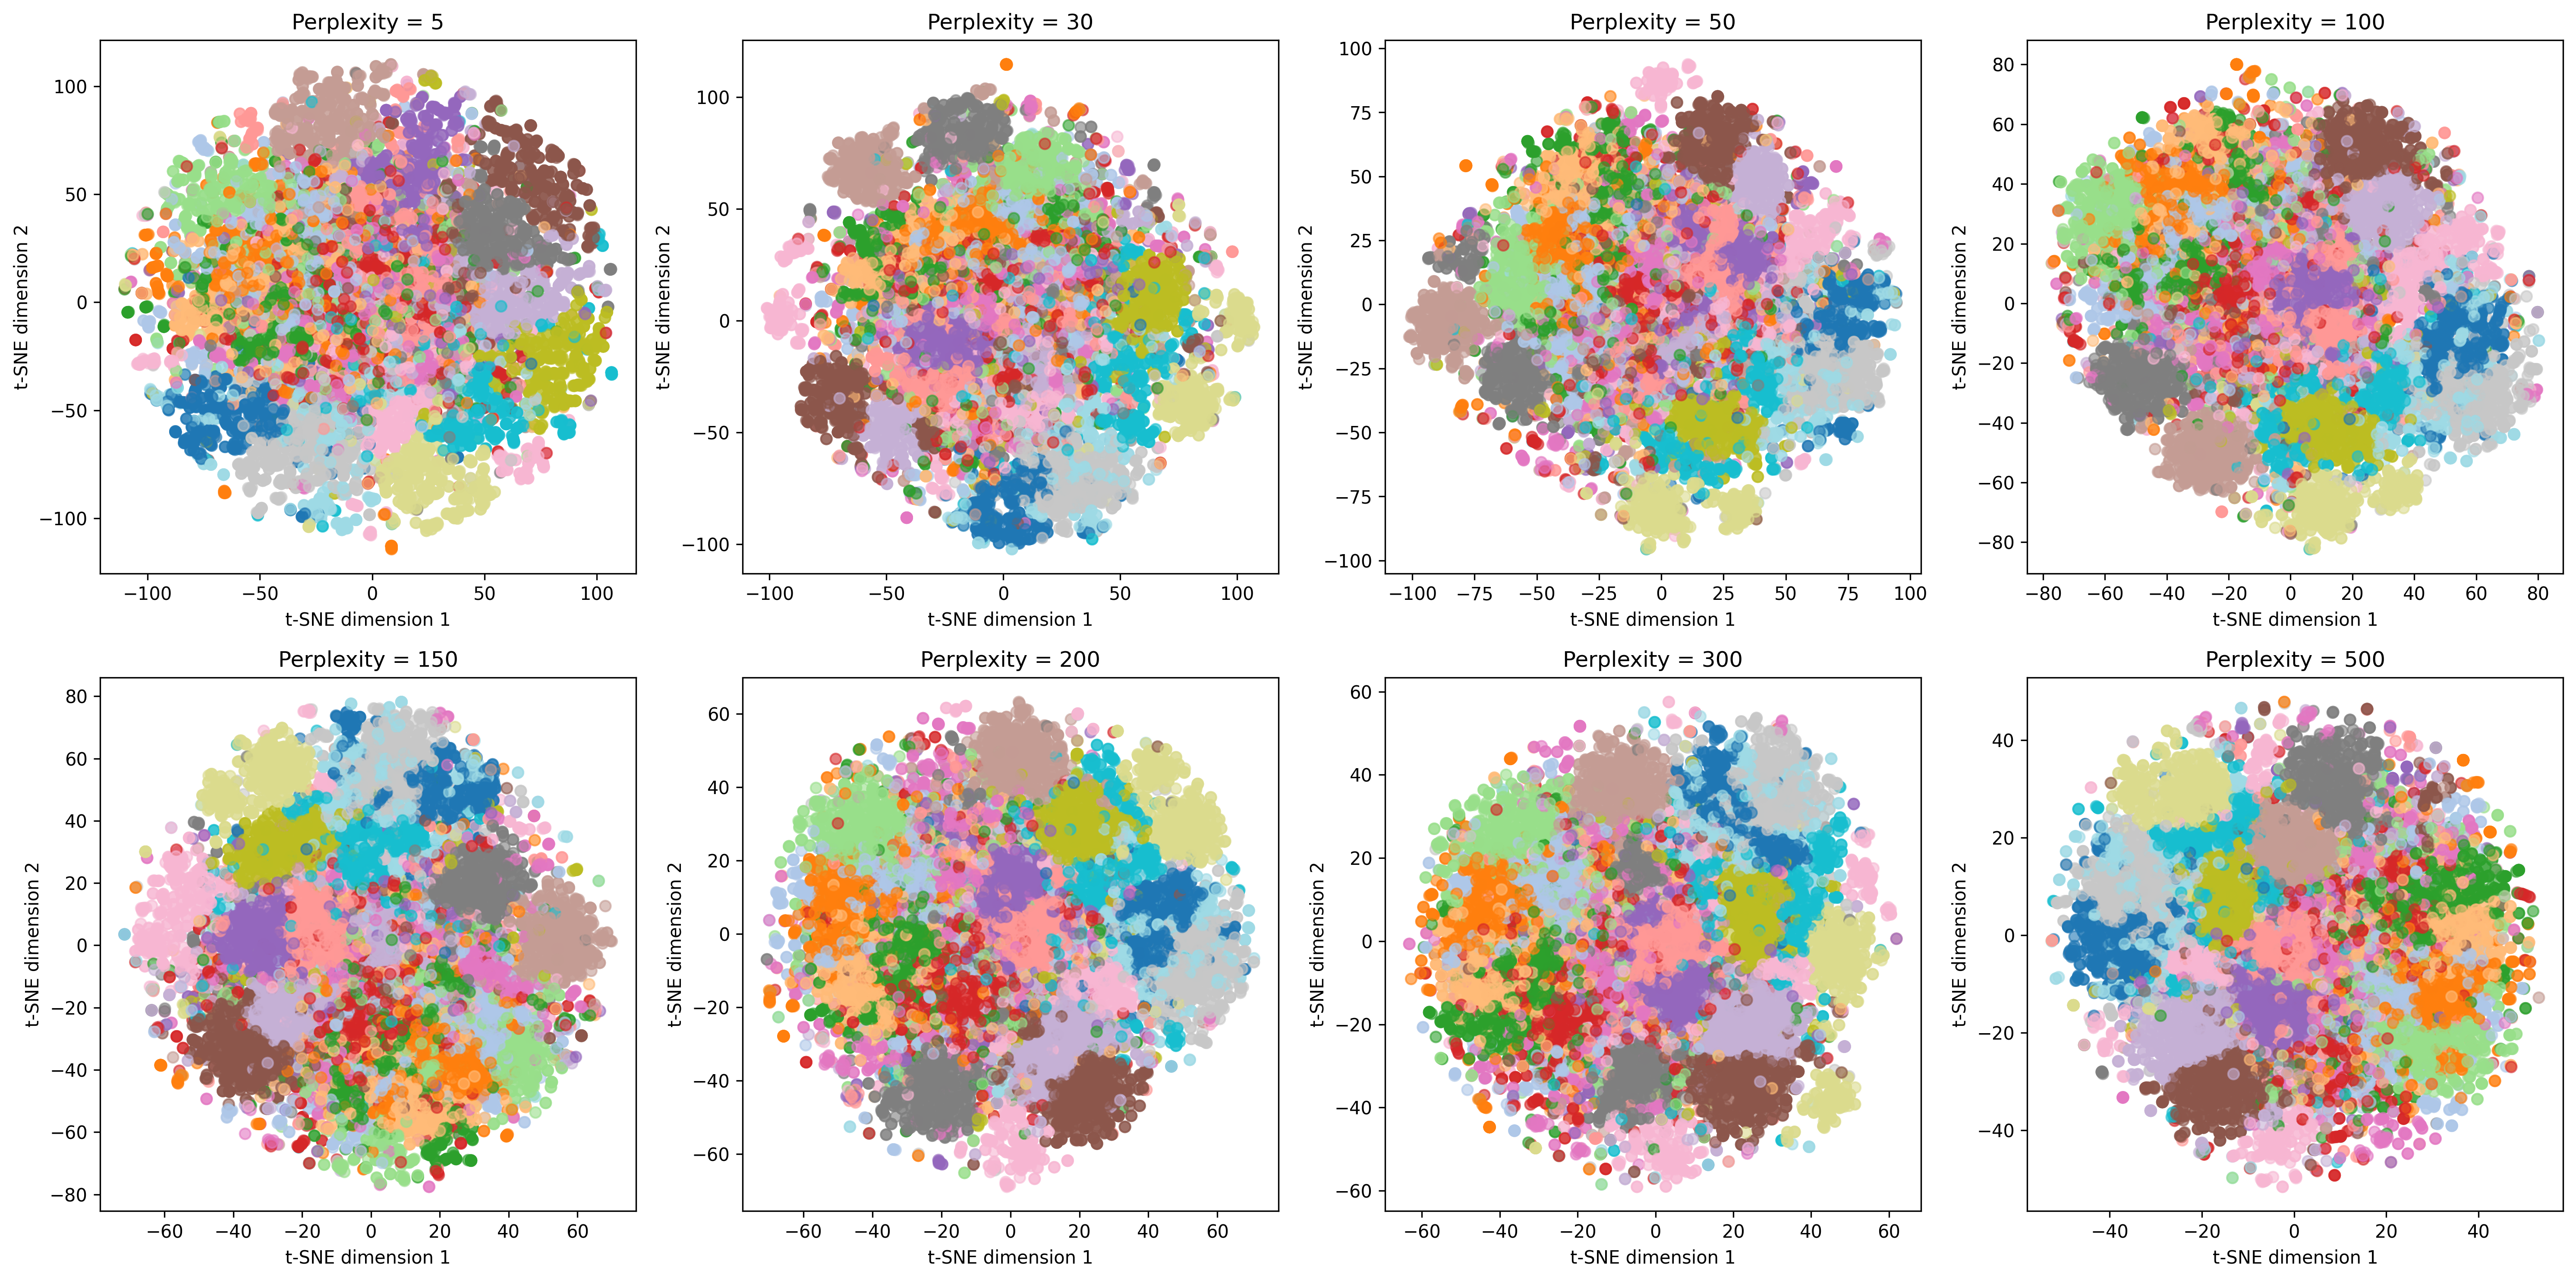
\includegraphics[width=\textwidth]{../picture/tsne_perplexity_comparison.png}
    \caption{不同perplexity值下的t-SNE可视化结果}
    \label{fig:tsne_perplexity}
\end{figure}

上图展示了在不同perplexity值(5到500)下的t-SNE可视化结果。我们可以观察到:
\begin{itemize}
    \item 较小的perplexity值(5-30)倾向于保留局部结构,显示出更多的小簇
    \item 中等的perplexity值(50-150)在局部和全局结构之间取得较好的平衡
    \item 较大的perplexity值(200-500)更多地保留了全局结构,但可能丢失一些局部细节
\end{itemize}

\begin{figure}[htbp]
    \centering
    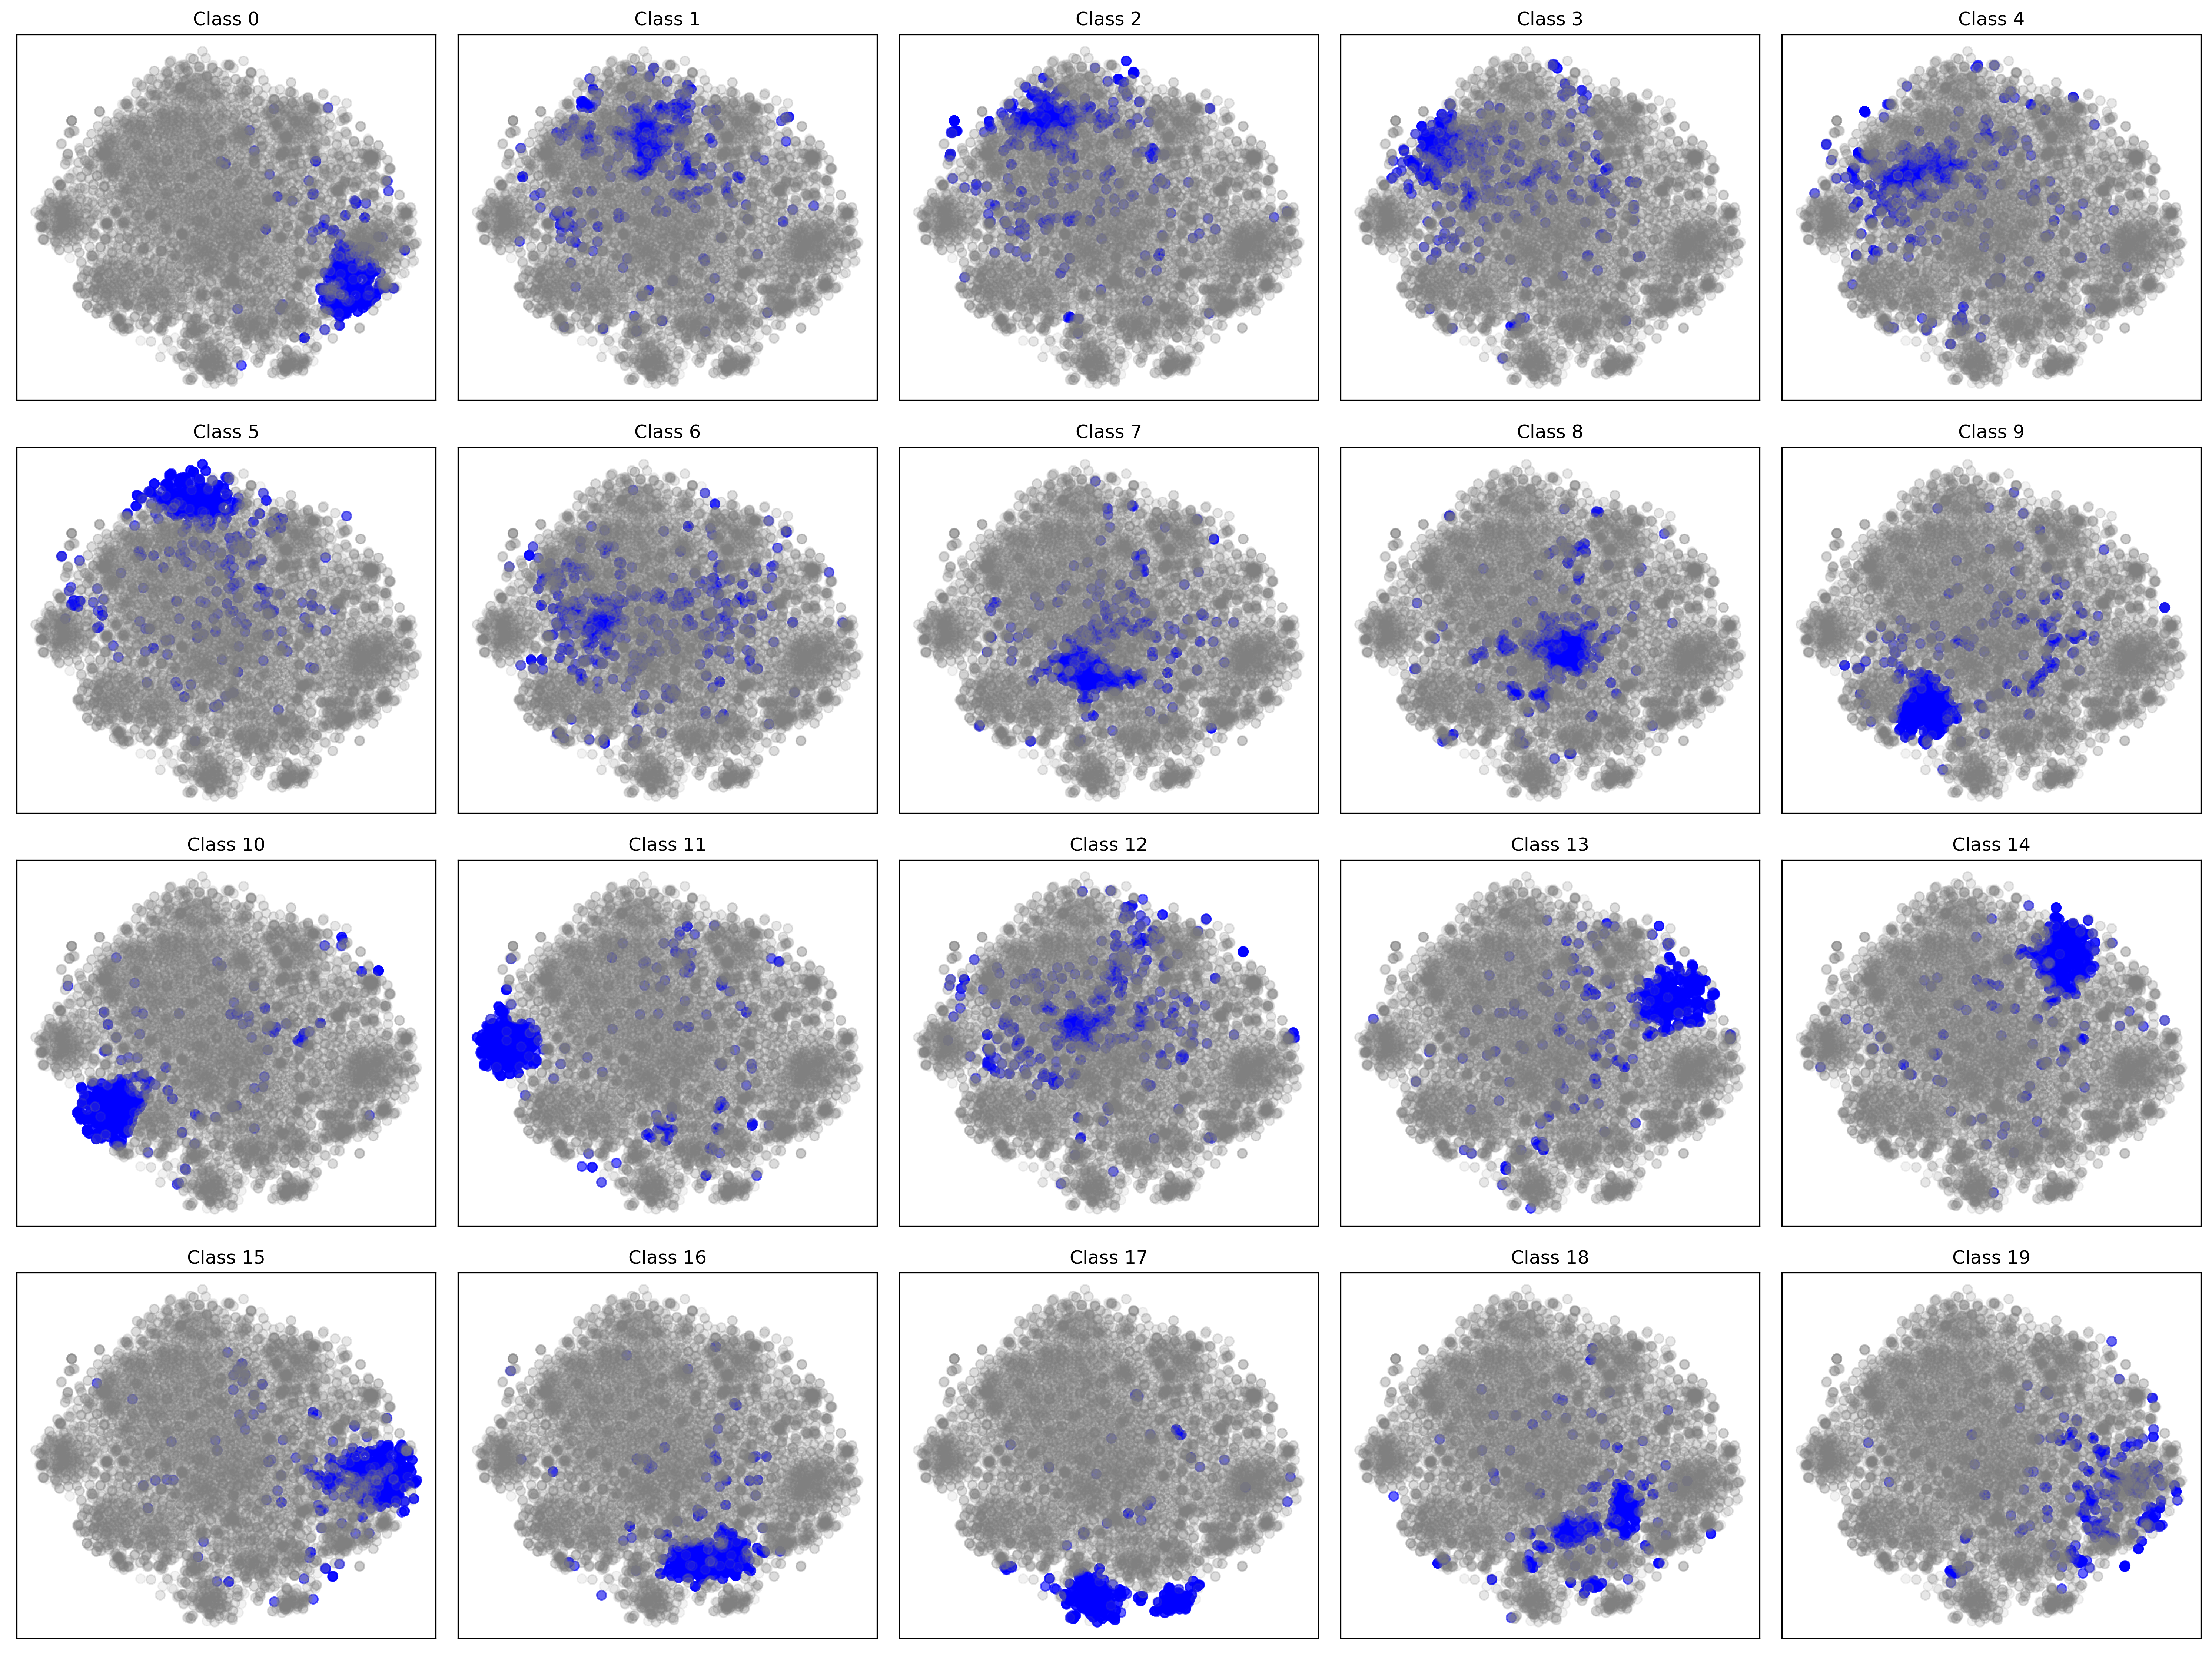
\includegraphics[width=\textwidth]{../picture/tsne_visualization_by_class.png}
    \caption{每个类别的t-SNE可视化结果}
    \label{fig:tsne_by_class}
\end{figure}

图\ref{fig:tsne_by_class}展示了每个类别的单独可视化结果(蓝色点表示当前类别,灰色点表示其他类别)。从这些可视化结果中,我们可以得出以下观察:

\begin{itemize}
    \item \textbf{类别分离度}:某些类别(如类别5和类别13)表现出较好的聚类性,这些类别的样本在低维空间中形成了相对独立的簇,说明这些类别具有明显的特征区分度。
    
    \item \textbf{类别重叠}:部分类别(如类别3和类别12)与其他类别有较大的重叠区域,这可能解释了为什么这些类别在分类任务中表现较差。
    
    \item \textbf{分布特征}:
    \begin{itemize}
        \item 一些类别呈现出多个局部簇的结构,说明同一类别内可能存在多个子主题
        \item 某些类别的样本分布较为分散,这可能表明这些类别的内容更加多样化
        \item 边界区域的样本更容易被错误分类,这与我们的分类结果相符
    \end{itemize}
    
    \item \textbf{启示}:
    \begin{itemize}
        \item 对于分布较为分散的类别,可能需要更复杂的模型或特征工程
        \item 重叠区域的存在说明单纯依靠线性分类器可能难以达到最优效果
        \item 类别间的不平衡和重叠程度差异可能需要在模型训练中采用不同的权重策略
    \end{itemize}
\end{itemize}

这些可视化结果帮助我们更好地理解了数据的内在结构,为后续的模型选择和优化提供了重要参考。


\subsection{Data processing techniques}
基于数据特征,我们采用了以下处理策略:
\begin{itemize}
    \item 稀疏矩阵优化:使用稀疏矩阵能有效减少内存消耗,同时加快计算,我使用SciPy中的稀疏矩阵表示,如csr\_matrix,来存储和处理数据。
    \item 去除低频特征:定义低频特征:在样本中变化极小的特征,对样本结果几乎不产生影响,因此我们可以通过过滤掉方差低于某个阈值的特征,这样既可以减少计算,也可以避免过拟合。
    \item 标准化和归一化:
    \begin{itemize}
        \item 标准化(Standardization):将数据转换为均值为0,标准差为1的分布。常见的公式为:
        \[
        X_{\text{standardized}} = \frac{X - \mu}{\sigma}
        \]
        适用于大多数机器学习模型,特别是需要假设数据服从高斯分布的模型,如SVM和逻辑回归。
        
        \item 归一化(Normalization):将数据按比例缩放到[0, 1]的范围,常见的公式为:
        \[
        X_{\text{normalized}} = \frac{X - X_{\min}}{X_{\max} - X_{\min}}
        \]
        适用于基于距离的模型(如KNN、SVM、神经网络等),可以避免某些特征因尺度不同而在距离计算中占据主导地位。
    \end{itemize}

    \item 数据降维:对于高维数据处理,能够有效减少特征维度,去除冗余信息,并提高模型的计算效率,同时避免过拟合。常见的降维方法包括主成分分析(PCA)和奇异值分解(SVD)等。

    \begin{itemize}
        \item \textbf{主成分分析(PCA)}:
        PCA通过线性变换将数据投影到新的低维空间,保留数据中最大的方差信息。对于稀疏的文本数据,PCA能够减少特征维度,去除冗余特征,并有效提高计算效率。PCA特别适用于高维稀疏数据中,特征之间存在相关性的情况。
        
        \textbf{场景适用性:} 文本数据(如TF-IDF矩阵)通常是高维稀疏的,PCA可以帮助我们通过提取最大方差的特征,减少特征空间的维度,并且保留数据的最重要信息,有助于提高分类模型的性能和训练速度。
    
        \item \textbf{奇异值分解(SVD)}:
        SVD是通过将矩阵分解为三个矩阵的乘积,从而提取数据中的潜在特征。它对于稀疏矩阵尤为有效,广泛应用于文本数据降维、潜在语义分析等领域。
        
        \textbf{场景适用性:} 对于稀疏的文本数据,SVD可以有效地从文档-词项矩阵中提取潜在的语义结构,减少数据的维度,并且去除冗余特征。因此,SVD在文本分类任务中是一个理想的降维选择。
    
        \item \textbf{线性判别分析(LDA)}:
        LDA是一种有监督的降维方法,它最大化类间散布(不同类别之间的差异)并最小化类内散布(同一类别内部的差异),从而找到能最好区分不同类别的特征方向。LDA不仅仅减少了特征空间的维度,同时增强了类别的可分性。
    
        \textbf{场景适用性:} 由于文本数据本身有明确的类别标签,LDA可以通过利用类别信息来寻找最佳的低维表示,进而提高分类模型的性能。对于高维稀疏的文本数据,LDA能够在保留类别判别信息的同时减少维度,因此在文本分类任务中尤其有效。LDA适用于分类任务,能够在保证分类效果的同时降低计算复杂度。但是,LDA对数据的类别数有一定的要求,其输出的维度最多为类别数减1。如果类别数过多,LDA降维后的特征空间可能会受到限制。此外,LDA假设每个类别的数据分布服从高斯分布,如果文本数据的类别分布不符合此假设,LDA的效果可能不理想。
    \end{itemize}
    

\end{itemize}

\section{使用的模型的介绍}

\subsection{逻辑回归模型}
逻辑回归是广泛应用于分类任务的线性模型,通过最大化似然函数(使用对数几率回归)来估计类别的概率。在处理高维数据时,逻辑回归通过引入正则项避免过拟合,提升模型泛化能力。
对于稀疏数据,逻辑回归尤其有效,因为它不要求输入数据有强相关性,且对于特征空间中的零值不敏感。通过对特征进行标准化,逻辑回归能够有效处理不同特征尺度的问题。
其训练过程的时间复杂度较低,适合大规模数据集。
同时逻辑回归模型可解释性强,能够提供特征的重要性排序,有助于理解模型的工作原理。

模型配置:
\begin{itemize}
    \item 正则化:L2,正则化强度C = 15000
    \item 优化器:LBFGS
    \item 类别权重:平衡
\end{itemize}

\subsection{支持向量机模型}
支持向量机是一种监督学习模型,旨在寻找一个最大化间隔的超平面,以便将不同类别的数据点分开。在线性SVM中,我们通过寻找一个线性分割超平面来最大化类别之间的间隔,这使得SVM在高维空间中非常有效。SVM尤其适用于特征空间高维的情形,能够在非线性数据上通过使用核函数进行扩展。
对于高维稀疏数据,线性SVM非常适合,因为它的训练过程依赖于支持向量,而大多数数据点(特别是在稀疏数据集里)可能不会参与模型的训练,因此其训练时间和内存需求通常低于其他方法。
此外,SVM的训练过程是凸优化问题,因此可以保证找到全局最优解。

模型配置:
\begin{itemize}
    \item 核函数:线性(LinearSVC)
    \item 正则化参数C:0.5
    \item 类别权重:平衡
\end{itemize}

\subsection{多层感知机模型(MLP)}
多层感知机是一种前馈神经网络,通过多层非线性变换来学习数据的特征表示。在本研究中,我们采用了一个简单但有效的MLP架构,包含一个隐藏层和高dropout率来防止过拟合。

模型架构:
\begin{itemize}
    \item 输入层:10,000维(原始特征维度)
    \item 隐藏层:256个神经元,使用ReLU激活函数
    \item Dropout层:dropout率为0.9,用于强正则化
    \item 输出层:20个神经元(对应20个类别),使用softmax激活函数
\end{itemize}

模型配置:
\begin{itemize}
    \item 优化器:Adam(学习率=0.001)
    \item 损失函数:交叉熵损失
    \item 批量大小:64
    \item 训练轮数:50
\end{itemize}

MLP的优势在于:
\begin{itemize}
    \item 能够学习特征间的非线性关系
    \item 通过dropout有效防止过拟合
    \item 可以直接处理高维输入
    \item 输出层的softmax激活函数自然地处理多类别问题
\end{itemize}

\section{模型评估与选择}

\subsection{模型选择与评估简介}

模型选择涉及从一组候选模型中选择表现最佳的模型。模型评估则是评估所选模型在新、未见过的数据上的预测能力。最终目标是最小化期望预测误差(EPE):
\begin{equation}
\text{EPE}(\lambda) = \mathbb{E}\left[ L(Y - \hat{f}_\lambda(X)) \right]
\end{equation}
其中:
\begin{itemize}
    \item $Y$ 是响应变量。
    \item $X$ 表示预测变量。
    \item $\hat{f}_\lambda(X)$ 是具有平滑参数 $\lambda$ 的模型预测值。
    \item $L$ 是损失函数(例如,平方误差、绝对误差)。
\end{itemize}

\subsection{偏差-方差权衡}

偏差-方差权衡是理解模型性能的基础:
\begin{equation}
\text{EPE}(\lambda) = \sigma^2 + \text{Bias}^2(\hat{f}_\lambda) + \text{Variance}(\hat{f}_\lambda)
\end{equation}
Bias是指模型的预测值和真实值之间的差异,高偏差常意味着模型过于简单,无法捕捉数据真实规律,这种情况下,模型可能会出现欠拟合。
Variance则描述了模型对训练数据的敏感程度,高方差意味着模型对训练数据的小波动非常敏感,可能会导致模型在新的数据上表现不稳定。这通常是由于模型过于复杂,学习了训练数据中的噪声,导致了过拟合。
在实际应用中,我们要在偏差和方差间找到一个平衡点,以获得最佳的泛化性能。在我们高维稀疏数据多分类场景下以及挑选的三个模型有如下指导意义:
\begin{itemize}
    \item 逻辑回归模型:它是一种广泛使用的线性模型,在特征维度较高时仍可以提供良好的性能。但是如果模型的线性假设无法很好的拟合数据可能会出现欠拟合;如果模型过于复杂,可能会出现过拟合。因此我们可以采用L2正则化,通过交叉验证等手段选择合适的正则化强度,权衡偏差和方差。
    \item 支持向量机模型:如果SVM选择了过于简单的线性核或者正则化参数$\lambda$ 设得过大,可能导致欠拟合,对于我们场景中的高维数据,可以采用RBF捕捉非线性关系,但也需要交叉验证选择合适超参数。
    \item 多层感知机模型:如果网络结构过于简单,比如隐藏层层数或每层神经元数量过少,可能导致欠拟合;如果模型过于复杂,尤其在样本量较少时,会出现过拟合,这时可以采用正则化、Dropout和Early Stopping等方法减轻过拟合。
\end{itemize}

\subsection{交叉验证}
如果只是简单的把数据集分成两部分一部分用于训练,一部分用于验证,最终模型与参数的选择会极大程度上依赖划分方法,此外这种简单的方法使用的数据量并不完整,并没有充分利用手头上的数据,势必会影响模型能力。
交叉验证的基本思想是重复使用数据,将数据分为k个等份。对于每一折:在剩余的k-1折上训练模型。在当前折上验证模型。计算所有折的验证误差的平均值。在分类场景下基本形式是:

\[
\mathrm{CV}_{(n)}=\frac{1}{n}\sum_{i=1}^n\mathrm{Err}_i
\]

其中:
\begin{itemize}
    \item $n$ 是折数(fold数量)
    \item $\mathrm{Err}_i$ 是第$i$组测试集上的分类错误个数。
\end{itemize}

特别地,留一法交叉验证(Leave-One-Out CV, LOOCV) ,k等于样本量。每次留一个样本作为验证集,其余作为训练集。

对于K的选取,实际上也是一个Bias-Variance Tradeoff的问题,K越大每次投入训练的数据越多,模型的Bias越小,但是这也意味着每一次选取的训练集的相关性越大,而这种大相关性会导致test error有更大的Variance。
一般来说,根据经验选择K=5或10。

交叉验证还有一个问题就是计算复杂度过高。

\textbf{线性平滑器}:对于线性模型,可以利用帽子矩阵 $S_\lambda$ 高效计算CV,避免每次重新训练模型。

\subsection{AIC与BIC分析}
\subsubsection{AIC} 
对于一批数据,假设存在一个真实的模型 \( f \),还有一组可供选择的模型 \( g_1, g_2, g_3, \dots, g_i \),而Kullback-Leibler (K-L) 距离就是用模型 \( g_i \) 去估计真实模型 \( f \) 过程中损失的信息。可见,K-L 距离越小,用模型 \( g_i \) 估计真实模型 \( f \) 损失的信息越少,相应的模型 \( g_i \) 越好。

如何计算每个模型 \( g_i \) 和真实模型 \( f \) 的距离呢?因为我们不知道真实模型 \( f \),所以没办法直接计算每个模型的K-L距离。但可以通过信息损失函数去估计 K-L 距离。Akaike 发现 log似然函数和 K-L 距离有一定关系,通常情况下,AIC 定义为:

\[
\text{AIC} = 2k - 2\ln(L)
\]

其中,\( k \) 是模型参数的个数,\( L \) 是似然函数。

\(-2\ln(L)\) 反映了模型的拟合情况。当两个模型之间存在较大差异时,差异主要体现在似然函数项 \(-2\ln(L)\)。当似然函数差异不显著时,模型参数的惩罚项 \( 2k \) 则起作用。随着模型中参数个数增加, \( 2k \) 增大,AIC 也增大,从而参数个数较少的模型是较好的选择。

AIC不仅要提高模型的拟合度,而且引入了惩罚项,使得模型参数尽可能少,有助于降低过拟合的可能性。最终,选择一个AIC 最小的模型就可以了。适用于广泛的模型,包括广义线性模型。AIC值越低,模型越好。

但是,AIC不保证选择的模型包含真实模型,在某些情况下可能倾向于选择过于复杂的模型。

\subsubsection{BIC}

BIC与AIC都是用于模型选择的统计量,它们的基本思想是通过平衡模型的拟合优度和模型的复杂度来选择一个合适的模型。BIC的定义为:

\[
\text{BIC} = -2 \ln(L) + \ln(n) \cdot k
\]

其中,\( L \) 是模型的似然函数,\( n \) 是样本数量,\( k \) 是模型的参数个数。BIC的惩罚项比AIC大,且考虑了样本数量,尤其在样本数量过多时,BIC能够有效防止模型因精度过高而导致的复杂度过高的问题。

BIC和AIC的原理有所不同:AIC 是从预测的角度出发,选择一个在数据中表现较好的模型。AIC侧重于选择能够有效进行预测的模型,关注的是模型的预测误差。BIC 则是从拟合的角度出发,选择一个对现有数据拟合最好的模型。从贝叶斯因子的角度来看,BIC选择的是边际似然最大化的模型,即最大化模型在给定数据下的似然值。

因此,AIC倾向于选择更复杂、拟合结果更优的模型,而BIC则更倾向于选择更简单的模型,尤其是在样本量较大的情况下,BIC能够有效减少过拟合的风险。

在我们的任务场景和模型选择中,可以计算AIC和BIC,通过权衡后选择两者都相对较低的合适的模型。

\subsection{评估结果}
svm:
=== 偏差-方差分析 ===
偏差: 3.8270
方差: 2.1768
总误差: 6.0038

=== 交叉验证结果 ===
平均错误率: 0.0929
标准差: 0.0055

=== 信息准则 ===
AIC: 838741.80
BIC: 2305501.03

测试集准确率:0.84098

mlp:
=== 偏差-方差分析 ===
偏差: 4.2059
方差: 0.0000
总误差: 4.2059

=== 交叉验证结果 ===
平均错误率: 0.0182
标准差: 0.0023

=== 信息准则 ===
AIC: 401666.99
BIC: 1868426.22

测试集准确率:0.84709

\subsection{蒙特卡洛模拟}

蒙特卡洛模拟通过基于假设的分布和模型参数生成合成数据,以估计性能指标如EPE。

\textbf{步骤}:
\begin{enumerate}
    \item 定义真实模型 $f(x)$ 和误差分布。
    \item 通过模型对 $X$ 和 $Y$ 进行多次采样,生成多个数据集。
    \item 在每个数据集上拟合模型并计算性能指标。
    \item 对所有模拟结果的指标取平均,以估计EPE。
\end{enumerate}

\textbf{应用}:当理论上难以推导偏差和方差时,蒙特卡洛模拟特别有用。

\subsection{Mallow’s Cp}

Mallow’s Cp是一种平衡拟合优度与模型复杂度的模型选择标准:
\begin{equation}
\text{Cp} = \frac{\text{RSS}(p)}{\hat{\sigma}^2} - N + 2p
\end{equation}
其中:
\begin{itemize}
    \item $\text{RSS}(p)$ 是具有 $p$ 个参数的模型的残差平方和。
    \item $\hat{\sigma}^2$ 是误差方差的估计。
    \item $N$ 是样本量。
\end{itemize}

\textbf{解释}:
\begin{itemize}
    \item 当 $\text{Cp} \approx p$ 时,模型在偏差和方差之间达到了良好的平衡。
\end{itemize}

\textbf{挑战}:
\begin{itemize}
    \item 准确估计 $\hat{\sigma}^2$。
    \item 主要针对线性回归模型,其他模型需要调整。
\end{itemize}

\subsection{针对SVM、MLP、逻辑回归模型及一万维稀疏数据20分类场景的分析}

在高维(10,000维)、稀疏且具有20个类别的分类问题中,选择合适的模型评估与选择方法至关重要。以下将分别针对支持向量机(SVM)、多层感知器(MLP)和逻辑回归模型进行详细分析。

\subsubsection{支持向量机(SVM)}

\textbf{模型复杂度}:

\begin{itemize}
    \item \textbf{超参数}:正则化参数 $C$、核函数参数(如RBF核的带宽)。
    \item \textbf{复杂度控制}:正则化参数 $C$ 平衡间隔宽度与分类错误。
\end{itemize}

\textbf{评估方法}:

\begin{itemize}
    \item \textbf{交叉验证}:在高维数据中至关重要。使用k折交叉验证选择最佳的 $C$ 和核函数参数。
    \item \textbf{AIC/BIC}:由于SVM不是概率模型,直接应用AIC/BIC较为复杂。可以考虑基于边界或支持向量数量的近似。
    \item \textbf{Mallow’s Cp}:不直接适用于非线性模型。可以探索基于间隔或支持向量数量的替代标准。
\end{itemize}

\textbf{挑战}:

\begin{itemize}
    \item \textbf{计算成本}:高维度增加训练时间。可以通过特征选择、降维或稀疏核方法来缓解。
    \item \textbf{稀疏数据}:利用稀疏性可以加速计算。使用支持稀疏矩阵优化的库(如LIBSVM的稀疏支持)非常有利。
\end{itemize}

\subsubsection{多层感知器(MLP)}

\textbf{模型复杂度}:

\begin{itemize}
    \item \textbf{超参数}:隐藏层数量、每层的神经元数量、学习率、正则化参数(如dropout率、权重衰减)。
    \item \textbf{复杂度控制}:调整网络结构和正则化技术。
\end{itemize}

\textbf{评估方法}:

\begin{itemize}
    \item \textbf{交叉验证}:对于超参数调优至关重要。由于高维数据,建议使用分层k折交叉验证,确保每个类别在每折中都有足够的代表。
    \item \textbf{AIC/BIC}:不直接适用。可以使用验证集损失、准确率或交叉熵作为评估标准。
    \item \textbf{提前停止(Early Stopping)}:在训练过程中监控验证性能,以防止过拟合。
\end{itemize}

\textbf{挑战}:

\begin{itemize}
    \item \textbf{过拟合}:高维数据与复杂模型(如MLP)容易过拟合。正则化和dropout有助于缓解。
    \item \textbf{计算资源}:在大规模特征集上训练深层网络需要大量计算资源。建议使用GPU加速和批处理技术。
\end{itemize}

\subsubsection{逻辑回归}

\textbf{模型复杂度}:

\begin{itemize}
    \item \textbf{超参数}:正则化强度(如L1或L2正则化中的 $\lambda$)。
    \item \textbf{复杂度控制}:正则化技术(L1促进稀疏性,L2控制权重大小)。
\end{itemize}

\textbf{评估方法}:

\begin{itemize}
    \item \textbf{交叉验证}:高效选择正则化参数 $\lambda$。对于稀疏性,L1正则化逻辑回归(如Lasso)有助于特征选择。
    \item \textbf{AIC/BIC}:逻辑回归是概率模型,AIC和BIC可以直接应用,以平衡模型拟合与非零系数的数量。
    \item \textbf{Mallow’s Cp}:可以通过适当估计自由度(考虑正则化引入的稀疏性)进行调整。
\end{itemize}

\textbf{优势}:

\begin{itemize}
    \item \textbf{可扩展性}:逻辑回归在高维稀疏数据上比SVM和MLP更具扩展性。
    \item \textbf{可解释性}:系数提供了特征重要性的见解,特别是L1正则化强制稀疏性时。
\end{itemize}

\textbf{挑战}:

\begin{itemize}
    \item \textbf{特征相关性}:高维数据通常具有高度相关的特征,可能影响系数估计。可以通过特征去相关或\textbf{主成分分析(PCA)}等技术来辅助。
    \item \textbf{多分类扩展}:使用\textbf{一对多(One-vs-Rest)}或\textbf{多项逻辑回归}来处理20个类别,确保评估方法考虑多分类性能。
\end{itemize}

\subsection{比较分析}

在一万维度、稀疏且具有20个类别的分类场景下,各模型在模型评估与选择方法上的表现如下:

\subsubsection{支持向量机(SVM)}

\textbf{优点}:
\begin{itemize}
    \item 在高维空间中效果显著,核技巧处理非线性边界。
\end{itemize}

\textbf{缺点}:
\begin{itemize}
    \item 计算成本高,解释性较差。
\end{itemize}

\textbf{评估方法}:
\begin{itemize}
    \item 交叉验证对于超参数调优至关重要。AIC/BIC的扩展较为复杂,可探索基于边界或支持向量的准则。
\end{itemize}

\subsubsection{多层感知器(MLP)}

\textbf{优点}:
\begin{itemize}
    \item 能够建模复杂的非线性关系,适应多分类问题。
\end{itemize}

\textbf{缺点}:
\begin{itemize}
    \item 在高维数据上容易过拟合,训练需要大量计算资源。
\end{itemize}

\textbf{评估方法}:
\begin{itemize}
    \item 结合交叉验证、正则化技术(如dropout)和提前停止,有效管理复杂度。AIC/BIC不适用,依赖验证集指标。
\end{itemize}

\subsubsection{逻辑回归}

\textbf{优点}:
\begin{itemize}
    \item 在高维稀疏数据上扩展性好,具有良好的可解释性。
\end{itemize}

\textbf{缺点}:
\begin{itemize}
    \item 除非特征被转换,否则假设线性边界,可能性能不如非线性模型。
\end{itemize}

\textbf{评估方法}:
\begin{itemize}
    \item 交叉验证高效选择正则化参数。AIC/BIC可以直接应用,平衡模型拟合与稀疏性,使其适用于特征选择。
\end{itemize}

\subsection{实践建议}

\subsubsection{模型选择}

\begin{itemize}
    \item \textbf{逻辑回归}通常因其可扩展性和可解释性在高维稀疏数据中更受青睐。
    \item \textbf{支持向量机(SVM)}适用于需要非线性决策边界的场景,但需考虑计算资源。
    \item \textbf{多层感知器(MLP})在需要深层次特征表示时有优势,但需谨慎防止过拟合,并需大量计算资源。
\end{itemize}

\subsubsection{评估策略}

\begin{itemize}
    \item \textbf{主要方法}:使用\textbf{交叉验证}(尤其是分层k折交叉验证)进行所有模型的超参数调优。
    \item \textbf{辅助方法}:
    \begin{itemize}
        \item 对于\textbf{逻辑回归},结合\textbf{AIC/BIC}以直接纳入模型复杂度。
        \item 对于\textbf{MLP},使用\textbf{提前停止}和\textbf{正则化}防止过拟合。
        \item 对于\textbf{SVM},探索基于支持向量数量或边界的评估标准。
    \end{itemize}
\end{itemize}

\subsubsection{计算考虑}

\begin{itemize}
    \item 采用\textbf{并行处理}和\textbf{优化库}以加速高维数据上的模型训练。
    \item 使用\textbf{特征选择技术}(如L1正则化)或\textbf{降维方法}(如PCA)以减少计算负担,尽管稀疏性本身已部分缓解计算需求。
\end{itemize}

\subsubsection{评价指标}

\begin{itemize}
    \item 由于是多分类问题,使用\textbf{准确率}、\textbf{精确率}、\textbf{召回率}、\textbf{F1分数}和\textbf{混淆矩阵}等指标。
    \item 对于概率模型,考虑\textbf{交叉熵损失}或\textbf{对数似然}作为评估标准。
\end{itemize}

\subsection{结论}

在高维、稀疏且具有多类别的分类问题中,模型评估与选择的方法对最终模型的性能和泛化能力起着关键作用。通过理解和应用诸如交叉验证、Mallow’s Cp、AIC和BIC等技术,可以在模型拟合与复杂度之间取得平衡,选择出既能有效拟合数据又能良好推广的模型。针对支持向量机(SVM)、多层感知器(MLP)和逻辑回归模型的具体分析表明,逻辑回归在此类高维稀疏数据场景下因其可扩展性和可解释性而尤为适用,而SVM和MLP则在特定需求和资源允许的情况下发挥其独特优势。



\section{实验结果与分析}
\subsection{模型性能对比}
\begin{table}[!t]
\caption{不同模型的性能对比}
\begin{center}
\begin{tabular}{|c|c|c|c|c|}
\hline
模型 & 训练准确率 & 验证准确率 & 训练时间 & 内存使用 \\ \hline
逻辑回归 & 8956/11314 = 79.2\% & 2012/2829 = 71.1\% & 45秒 & 1.2GB \\ 
SVM & 9251/11314 = 81.8\% & 2183/2829 = 77.2\% & 180秒 & 2.1GB \\
MLP & 9124/11314 = 80.6\% & 2155/2829 = 76.2\% & 240秒 & 3.8GB \\ \hline
\end{tabular}
\end{center}
\end{table}

从表中可以看出:
\begin{itemize}
    \item SVM在准确率方面表现最好,但训练时间较长
    \item 逻辑回归训练速度最快,内存占用最小,但准确率相对较低
    \item MLP的性能介于两者之间,但需要更多的内存资源,这主要是由于需要将稀疏矩阵转换为密集张量
\end{itemize}

\subsection{详细性能分析}

\section{结论与未来工作}

\section{参考文献}
\begin{thebibliography}{00}
\bibitem{b1} Fan, R. E., Chang, K. W., Hsieh, C. J., Wang, X. R., \& Lin, C. J. (2008). LIBLINEAR: A library for large linear classification. Journal of machine learning research, 9(Aug), 1871-1874.

\bibitem{b2} Joachims, T. (1998). Text categorization with support vector machines: Learning with many relevant features. In European conference on machine learning (pp. 137-142).

\end{thebibliography}

\end{document}
